\subsection{Crossing BT}
\label{sec:Crossing-BT-impl}
    In this tree, the main decision-making of the road crossing is located. It is the third sub-tree to be ticked and the only one to be ticked repeatedly.\\
    In multiple nodes, we will use information about the detected vehicles and collision parameters for each vehicle. Therefore, we must first define the data structures used to store this information.\\\\
    \bfc{Vehicle data}\\
        The data structure for storing the information about the detected vehicles is defined in \ref{lst:vehicle_data}.\\
        The first struct \texttt{vehicle\_info} stores the information about the single detected vehicle. The position of the vehicle is expressed in relation to the robot's frame. The robot frame means the center of the robot is the origin of the coordinate system. The $x$-axis points forward from the robot, and the $y$-axis points to the right.\\
        The other options for expressing the position of the vehicle is in the global coordinate system or in the coordinate system of the road. The global coordinate system is defined by the GPS. The road coordinate system would be defined by the robot's position at the beginning of the crossing.\\
        We can use the coordinate system defined by the robot's current position for several reasons. Firstly, because the calculations are done periodically, and the results are only relevant for the current time step. We expect to obtain new information about the vehicles with a frequency of $5\:\si{\Hz}$. And secondly, it simplifies the process, as the vehicle positions are already expressed in the robot's frame.\\
        The second struct \texttt{vehicles\_data} stores the \texttt{vehicle\_info} structs of all detected vehicles.\\\\
    \bfc{Collision data}\\
        The data structure for storing the collision parameters has the definition in \ref{lst:collision_data}.\\
        The first struct \texttt{collision\_data} is used to store the collision parameters for a single vehicle.\\
        The velocities required for the robot to make contact with the front or back of the vehicle are stored in the variables \texttt{v\_front} and \texttt{v\_back}, respectively. Figure \ref{fig:collision} shows the contact points we calculate the velocities for. The figure is more thoroughly explained in the next part.\\
        The \texttt{collide} variable is a boolean value that tells us if the robot will collide with the vehicle. It is calculated based on the current velocities of the robot and the vehicle.\\
        The second struct \texttt{collisions\_data} stores the information about collisions with all detected vehicles.\\\\
    \bfc{Used units}\\
        We use these units for the measured and calculated parameters:
        \begin{itemize}
            \item \textbf{Position} -- meters $[\si{\m}]$
            \item \textbf{Time} -- seconds $[\si{\s}]$
            \item \textbf{Velocity} -- meters per second $[\si{\m\per\s}]$
            \item \textbf{Acceleration} -- meters per second squared $[\si{\m\per\square\s}]$
            \item \textbf{Dimensions} -- meters $[\si{\m}]$
        \end{itemize}
    \bfc{Calculating the collision parameters}\\
        First, we need to state the assumptions we are making in order to simplify the calculation.\\
        The first assumption is about the coordinate system we are using. We are using the robot's frame, where the robot's center is the system's origin, and all the positions are expressed in relation to this origin. The $x$-axis points forward, and the $y$-axis points to the right. The reasons for the validity of this assumption were stated earlier.\\
        The second assumption is about the movement of the robot. We assume the robot is moving in a straight line with constant velocity. This is reasonable as we want the robot to be as predictable as possible, so we do not want to move the robot to the side. The assumption about the constant velocity, meaning the acceleration is zero, is also reasonable. The speeds the robot can achieve are much lower than the robot's acceleration, which can, therefore, be neglected.\\
        The third assumption is about the movement of the vehicle. We assume the vehicle's acceleration is constant. This is a reasonable simplification as the calculation is done periodically with a high enough frequency.\\
        The fourth assumption is that we will calculate the collision only in two dimensions. This is reasonable as the $z$-axis will not impact the occurrence of a collision. Moreover, the area over which the collision can occur is relatively small. Therefore, any terrain deviations will not significantly impact the collision.\\\\
        Figure \ref{fig:collision} depicts a schematic view of the collision and figure \ref{fig:collided} shows the collision in the collision points. There are two contact points, both on the robot and the vehicle. The first one (blue) is the point where the robot is going to collide with the front of the vehicle. The second one (red) is the point where the robot is going to collide with the back of the vehicle.\\
        \begin{figure}[ht]
            \centering
            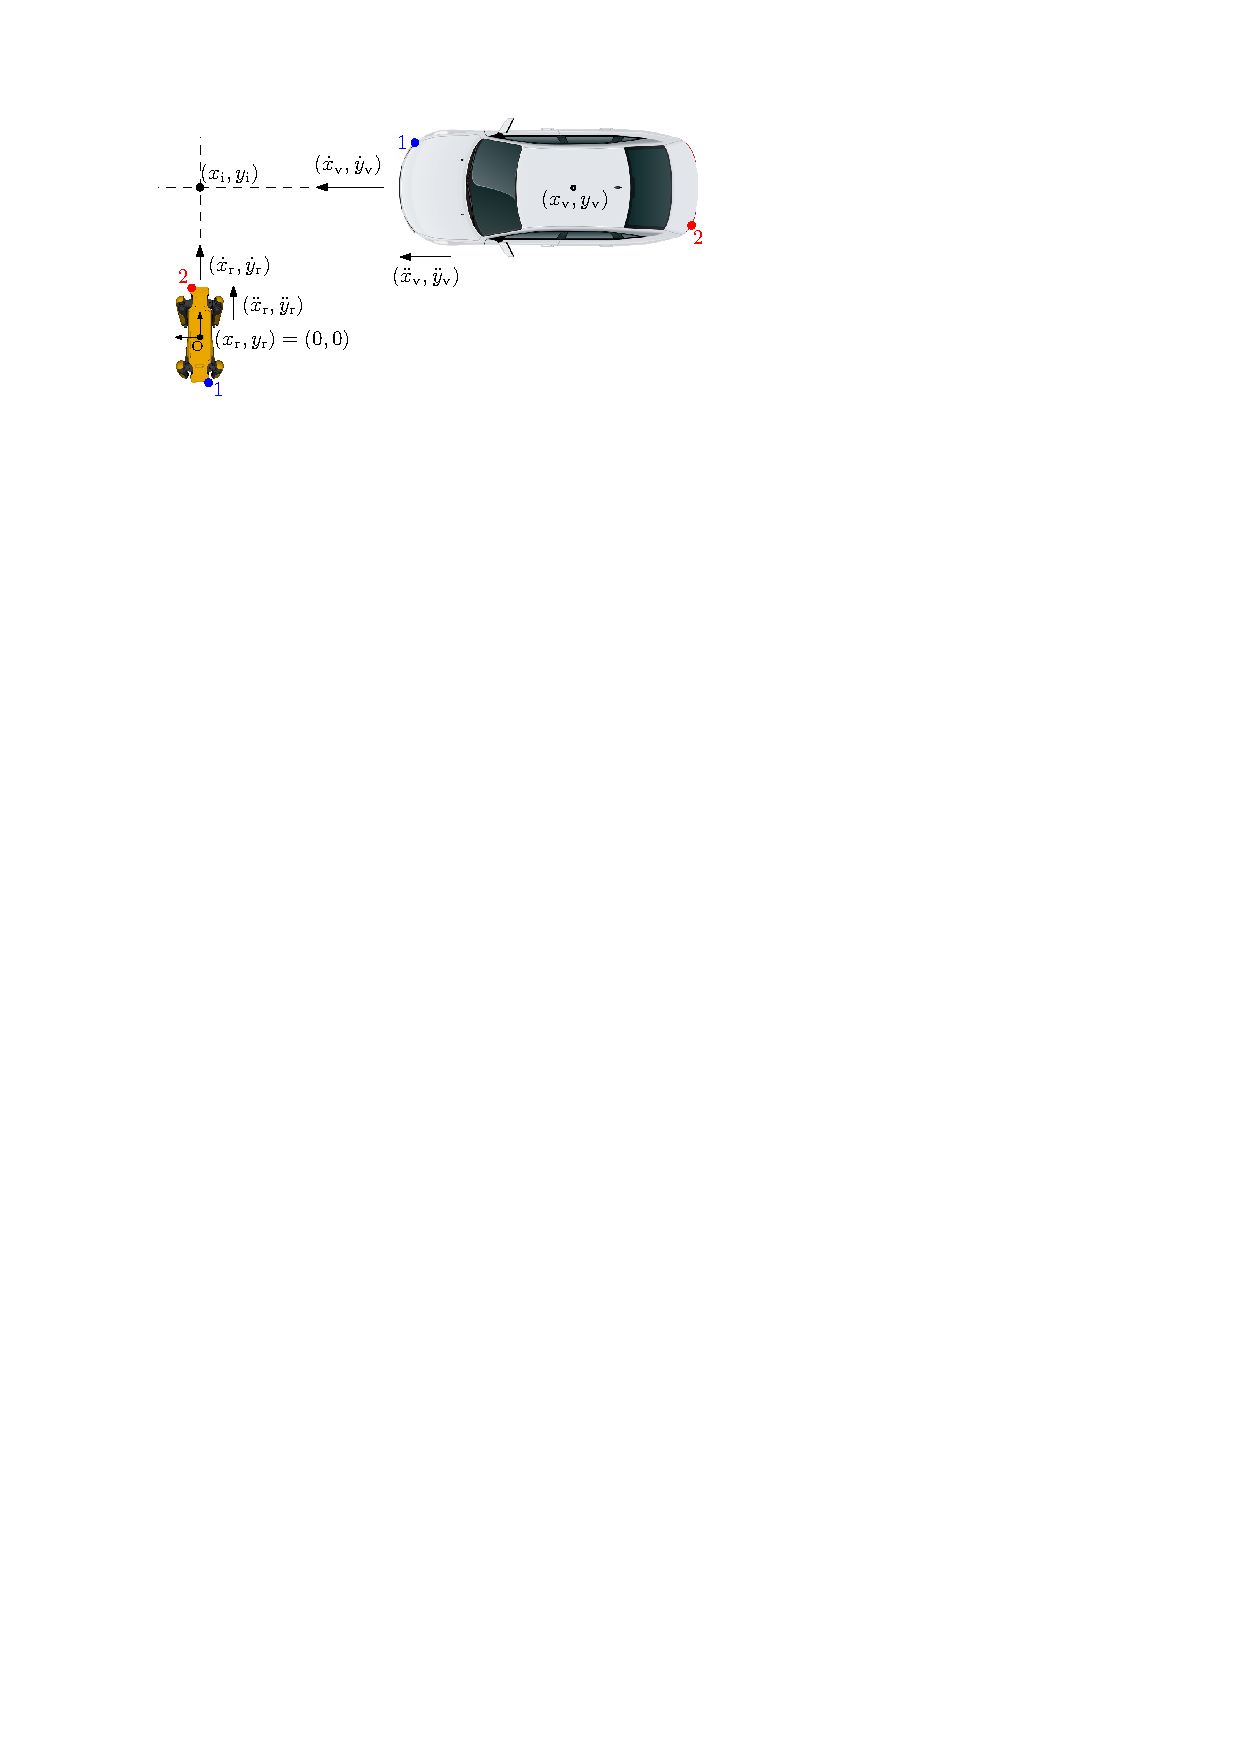
\includegraphics[height=6cm]{images/collision.pdf}
            \caption{Visualization of collision points, coordinate system, and vehicle parameters.}
            \label{fig:collision}
        \end{figure}
        \begin{figure}[ht]
            \centering
            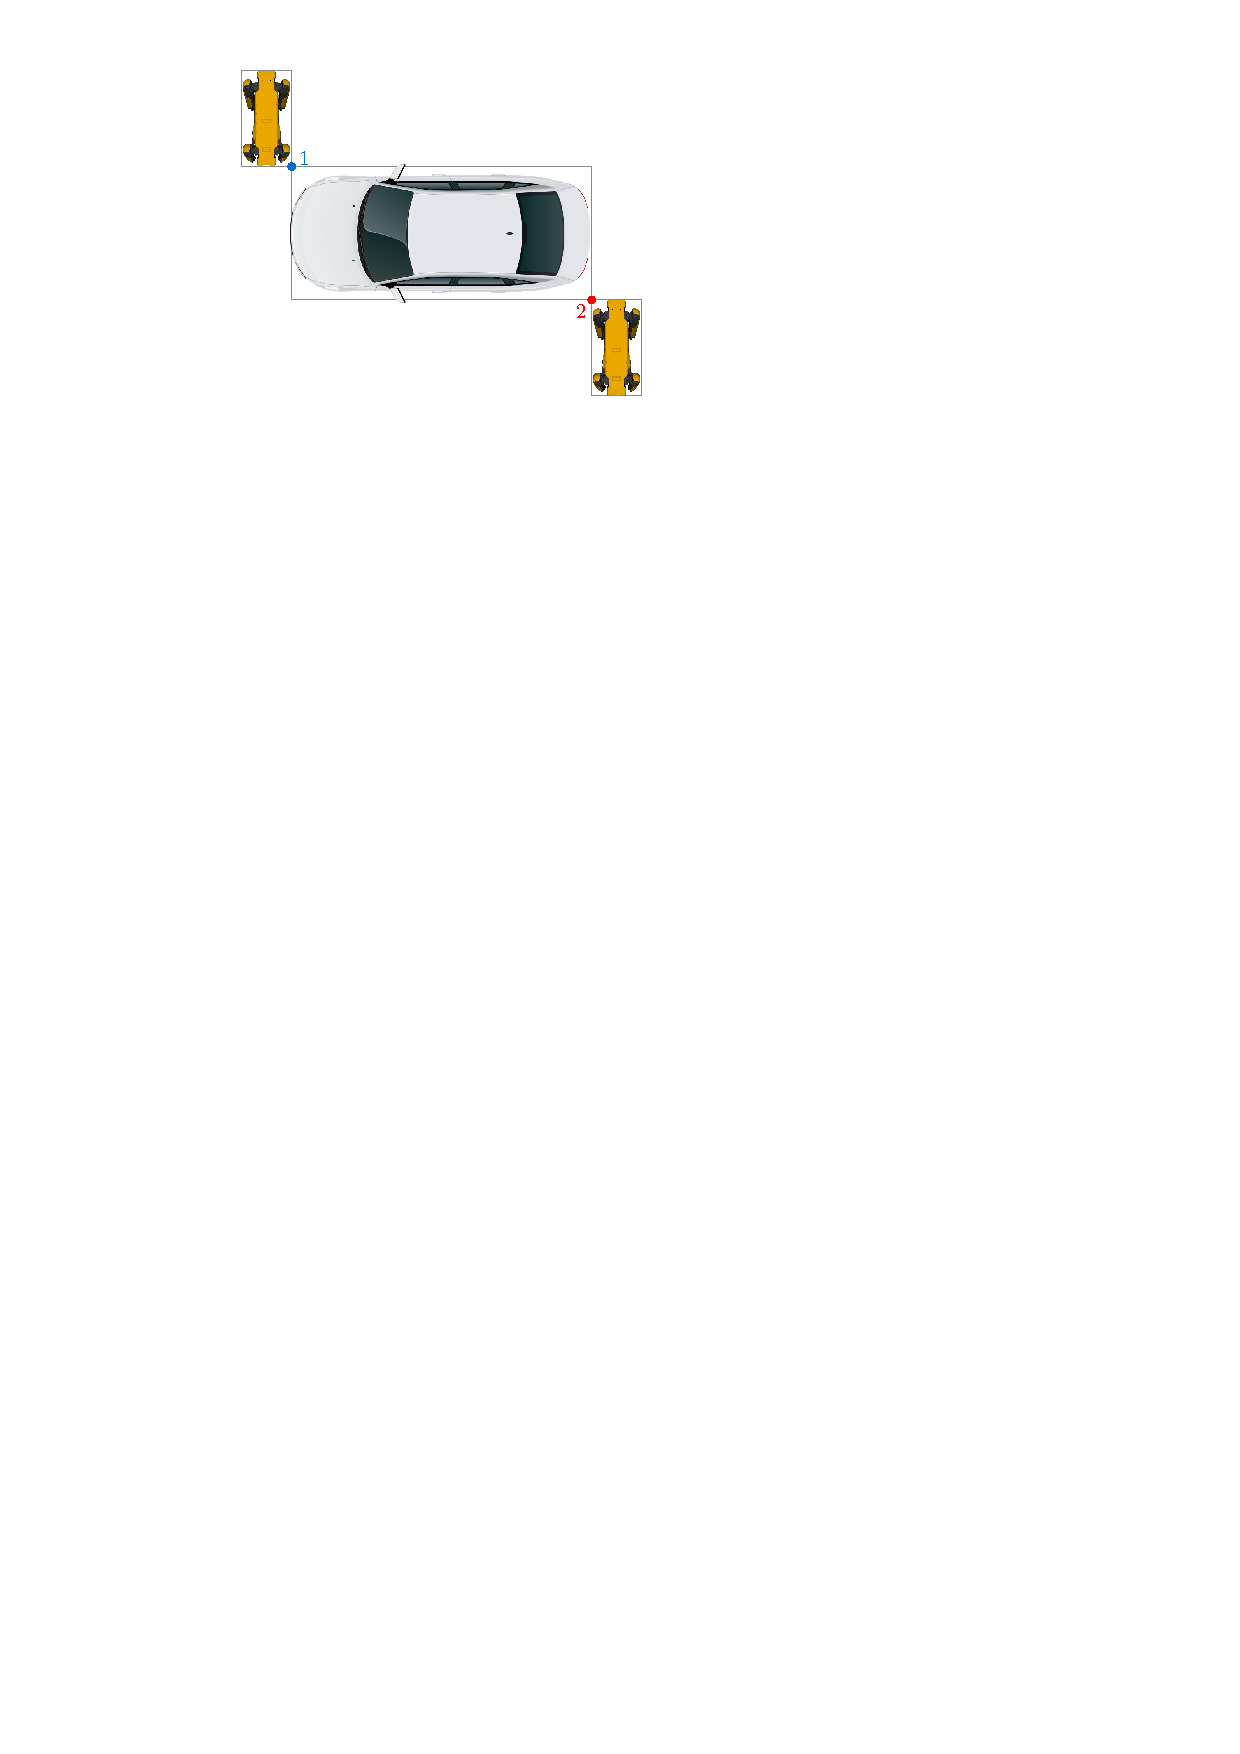
\includegraphics[height=7cm]{images/collided.pdf}
            \caption{Visualization of the collision in collision points.}
            \label{fig:collided}
        \end{figure}
        \noindent For the first point, we calculate the velocity \texttt{v\_front}. This velocity depicts the minimal speed of the robot to cross in front of the vehicle. We calculate the velocity \texttt{v\_back} for the second point. This velocity depicts the maximal speed of the robot to cross behind the vehicle.\\
        The subscript \texttt{r} is used for the parameters of the robot, and the subscript \texttt{v} is used for the parameters of the vehicle.\\
        The calculation is divided into three parts. In the first part, we determine the starting positions of the robot and the vehicle. In the second part, we calculate the time when the vehicle will reach the intersection point $(x_{\rm{i}}, y_{\rm{i}})$. And in the last part, we calculate the velocities for the robot to collide with the vehicle.\\\\
        The first part is necessary as the coordinates of both the robot and the vehicle are at the center of their respective bodies. We must move the starting points concerning the robot's and vehicle's length and width. The starting points for the robot are calculated using these equations:
        \begin{align}
            x_{\rm{r,f}} &= \frac{l_{\rm{r}}+w_{\rm{v}}}{2},\\
            x_{\rm{r,b}} &= -\frac{l_{\rm{r}}+w_{\rm{v}}}{2},\\
            y_{\rm{r,f}} &= y_{\rm{r,b}} = 0,
        \end{align}
        where $l_{\rm{r}}$ is the length of the robot and $w_{\rm{v}}$ is the width of the vehicle.\\
        The starting points for the vehicle are calculated as follows:
        \begin{align}
            x_{\rm{v,f}} &= x_{\rm{v}} + \frac{l_{\rm{v}}+w_{\rm{r}}}{2}\cos{(\varphi_{\rm{v}})},\\
            x_{\rm{v,b}} &= x_{\rm{v}} - \frac{l_{\rm{v}}+w_{\rm{r}}}{2}\cos{(\varphi_{\rm{v}})},\\
            y_{\rm{v,f}} &= y_{\rm{v}} + \frac{l_{\rm{v}}+w_{\rm{r}}}{2}\sin{(\varphi_{\rm{v}})},\\
            y_{\rm{v,b}} &= y_{\rm{v}} - \frac{l_{\rm{v}}+w_{\rm{r}}}{2}\sin{(\varphi_{\rm{v}})},
        \end{align}
        where $\varphi_{\rm{v}} = \arctan{\left(\frac{\dot{y}_{\rm{v}}}{\dot{x}_{\rm{v}}}\right)}$ is the angle of the vehicle, $l_{\rm{v}}$ is the length of the vehicle and $w_{\rm{r}}$ is the width of the robot.\\
        We put the width of the robot to calculate the vehicle's starting points and vice versa because we want to flatten objects in one dimension. This is done to simplify the calculation of the intersection point of the robot's and vehicle's trajectory.\\
        The second part of the calculation is further divided into two parts. The reason is that there are two possible scenarios for the calculation. We will use the general equation of motion \cite{equation_motion} for both calculations.\\
        In the first scenario, the vehicle's acceleration in the $y$-axis is zero. That means we can calculate the time using the following equations:
        \begin{align}
            t_{\rm{f}} = -\frac{y_{\rm{v,f}}}{\dot{y}_{\rm{v}}},\\
            t_{\rm{b}} = -\frac{y_{\rm{v,b}}}{\dot{y}_{\rm{v}}}.
        \end{align}
        In the second scenario, the acceleration of the vehicle in the $y$-axis is non-zero. This scenario is more probable, as vehicles rarely drive at a constant speed. In this case, the time is calculated in the following way:
        \begin{align}
            t_{\rm{f},1,2} = \frac{-\dot{y}_{\rm{v}}\pm\sqrt{\dot{y}_{\rm{v}}^2-2\ddot{y}_{\rm{v}}y_{\rm{v,f}}}}{\ddot{y}_{\rm{v}}},\\
            t_{\rm{b},1,2} = \frac{-\dot{y}_{\rm{v}}\pm\sqrt{\dot{y}_{\rm{v}}^2-2\ddot{y}_{\rm{v}}y_{\rm{v,b}}}}{\ddot{y}_{\rm{v}}}
        \end{align}
        There are two possible solutions for each time. The reason is that the vehicle may be decelerating and therefore change the direction of its travel. The interpretation of the results and the selection of the correct solution is discussed in the next section.\\
        The last part of the calculation is the calculation of the velocities. First, we need to calculate the position of the vehicle in the $x$-axis at the time of the collision. We use the general equation of motion with $t_{0}=0\:\rm{s}$:
        \begin{align}
            x_{\rm{i,f}} &= x_{\rm{v,f}} + \dot{x}_{\rm{v}}t_{\rm{f}} + \frac{1}{2}\ddot{x}_{\rm{v}}t_{\rm{f}}^2,\\
            x_{\rm{i,b}} &= x_{\rm{v,b}} + \dot{x}_{\rm{v}}t_{\rm{b}} + \frac{1}{2}\ddot{x}_{\rm{v}}t_{\rm{b}}^2.
        \end{align}
        Now we can calculate the velocities for the robot.
        \begin{align}
            \dot{x}_{\rm{r,f}} &= \frac{x_{\rm{i,f}}-x_{\rm{r,b}}}{t_{\rm{f}}},\\
            \dot{x}_{\rm{r,b}} &= \frac{x_{\rm{i,b}}-x_{\rm{r,f}}}{t_{\rm{b}}}.
        \end{align}
        The calculated velocities may be positive or negative. The interpretation is explained in the following section.\\\\
    \bfc{Interpretation of the calculated collision parameters}\\
        We will divide this section into two parts. The first part is the interpretation of the calculated time. The second part is the interpretation of the calculated velocities.\\\\
        If the calculated time is positive, the intersection point of the robot's and vehicle's trajectory is in the future. This means that the robot can collide with the vehicle without either of them changing the direction of travel.\\
        If the calculated time is negative, it means that the intersection point of the robot's and vehicle's trajectory is in the past. This means that the robot can collide with the vehicle, but only if the vehicle or the robot, depending on the situaion, would change its direction of travel.\\
        The time can also be zero. This means that the robot and vehicle already collided. Therefore, we do not expect such time to arise as a result of the calculation.\\
        We may have up to two solutions when calculating the times for non-zero acceleration in the $y$-axis. If we have none, the robot's and the vehicle's trajectories do not intersect.\\
        If we have one solution, the robot's and the vehicle's trajectories intersect once. The interpretation is that the vehicle is decelerating and will stop at the intersection point and then start reversing.\\
        If we have two solutions, the robot's and the vehicle's trajectories intersect two times. Multiple intersections could have several physical interpretations. We can interpret this as the vehicle decelerating, and therefore, changing the direction of travel after passing the intersection point. We can also interpret this as the vehicle accelerating, and therefore, the second time of the intersection is likely negative.\\
        When choosing the calculated time, we will use the following criteria. If both times are positive, we will use the shorter time. If both times are negative, we will use the larger time (the time that is closer to the present). If one time is positive and the second is negative, we will use the time with smaller absolute value.\\
        The velocities can also be positive or negative. The interpretation is similar to the one of time. Positive velocity means moving forward, while negative velocity means moving backward. It the resulting velocity was calculaed using negative time, than it also must be negative.\\
        While it may seem irrelevant to calculate the time and velocity for backward movement, it is essential. This is because there is a possibility that another vehicle may be in motion, which could result in a collision with the robot. In that case, the robot will have to move backward to avoid the collision, and we need to be able to set the correct backward velocity to not collide with the first vehicle.\\\\
    \bfc{GetCars -- action node}\\
        The action node \texttt{GetCars} obtains information about the detected vehicles. The detection node was not yet implemented when this thesis was written. Therefore, we will use the \texttt{GetCars} node to simulate the detection of vehicles.\\
        We will subscribe to the topic \texttt{/road\_crossing/injector}. We will publish this topic from a separate node designed solely to simulate the detection node.\\
        The information about the detected vehicles will be stored in a static variable for later use. The variable is of the format shown in listing \ref{lst:vehicle_data}.\\\\
    \bfc{CarsInTrajectory -- condition node}\\
        This node is important for optimizing the flow of ticks in our behavior tree. The node is responsible for checking if there are any detected vehicles. We do not need to go through the calculation and decision-making if there are no vehicles. This speeds up the completion of this run of the BT and allows us to start the next run sooner.\\\\
    \bfc{NotStarted -- condition node}\\
        This node is responsible for checking if the movement across the road has been started. If it has not, we need to start the movement. If it has, we may continue with it.\\\\
    \bfc{StartMovement -- action node}\\
        This node is responsible for starting the movement across the road. We will set the maximal forward linear velocity to our inner static variable. This variable is responsible for storing the current velocity. The maximal velocity is chosen based on the maximal velocity of the robot used.\\\\
    \bfc{MoveFwdFull -- action node}\\
        This node is used when no vehicles are detected, and therefore, we want to move the robot across the road as fast as possible. We publish the maximal forward linear velocity to the topic \texttt{/nav/cmd\_vel}.\\\\
    \bfc{CalculateCollision -- action node}\\
        In this node, we will calculate the collision parameters. We will use the formulas described earlier. The results will be stored in the inner static variables.\\
        This node will run the calculation for each vehicle independently. As each vehicle has its ID, we will use it to differentiate between them. This ID will also be used to delete all the results from the inner static variable when the vehicle is no longer detected.\\\\
    \bfc{MoveFwd -- action node}\\
        This node is used when vehicles are detected, and a forward movement is possible. We will publish the forward velocity to the topic \texttt{/nav/cmd\_vel}. The forward velocity is determined from the calculated velocities from the \texttt{CalculateCollision} node. We will set the maximal forward velocity while avoiding collisions.\\\\
    \bfc{MoveBwd -- action node}\\
        When the system detects the presence of other vehicles and determines that a backward movement is required, this node comes into play. To enable backward movement, we will publish the relevant velocity information to the topic \texttt{/nav/cmd\_vel}. The specific velocity will be calculated using the output from the \texttt{CalculateCollision} node. We will set the minimum backward velocity such that collisions are avoided.\\\\
    \bfc{StopMovement -- action node}\\
        This node is used when there is no possible movement forward without the robot colliding with a vehicle, and movement back is unnecessary or would also result in a collision. This node is also used as an emergency stop in case a movement was requested but no velocity could be chosen. We will stop the robot by publishing zero velocity to the topic \texttt{/nav/cmd\_vel}.\\\\
    \bfc{CollisionFwdMove -- condition node}\\
        This node is used to determine whether there are vehicles in front of the robot in such a position and velocity that the robot would collide with them if it moved forward.\\\\
    \bfc{CollisionBwdMove -- condition node}\\
        Same as the previous node, this one is used to determine whether there are vehicles in such a position and velocity that the robot would collide with them if it moved backward.\\\\
    \bfc{CollisionOnStop -- condition node}\\
        As the two condition nodes before, this node is used to determine whether there are vehicles in such a position and velocity that the robot would collide with them if we were to stop the robot.\\\\
    \bfc{CrossingFinished -- condition node}\\
        In this node, we check the current position of the robot. If the distance of the current position from the middle of the road is greater than half of the width of the road, we consider the crossing finished.\\
        Another condition for finishing the crossing is if the robot's distance from the starting point is greater than the width of the road.\\
        Having both of these conditions is beneficial, as the robot's position may be imprecise.
